\documentclass{CE295_HW_template}

\newcommand{\hmwkNum}{1}
\newcommand{\hmwkTitle}{HW \hmwkNum: Battery Modeling, Analysis, and Simulation}
\newcommand{\hmwkAuthorName}{Carlin Liao}
\newcommand{\SID}{24358933}

\title{
\vspace{-0.5cm}
\textbf{\hmwkTitle}
\author{} % Leave this blank
\date{} % Leave this blank
\vspace{-1cm}
}

%% Do not edit unless you really know what you are doing.
\documentclass[english]{article}
\usepackage[T1]{fontenc}
\usepackage[latin9]{inputenc}
\usepackage{textcomp}
\usepackage{relsize}

\makeatletter

%%%%%%%%%%%%%%%%%%%%%%%%%%%%%% User specified LaTeX commands.
\def\labnb{0}
\usepackage{hyperref} 
\usepackage{ulem}
\usepackage{latexsym}
\usepackage{amssymb}
\usepackage{amsmath}
\usepackage{amsfonts}
\usepackage{color, colortbl}
\usepackage{graphicx}
\usepackage{lastpage}
\usepackage[framed,numbered,autolinebreaks,useliterate]{mcode}

\newcommand{\red}[1]{{\color{red}#1}}
\newcommand{\blue}[1]{{\color{blue}#1}}
\newcommand{\green}[1]{{\color{green}#1}}

%%%%%%%%%%%%%%%%%%%%%%%%%%%%%%%%%%%%%%%%%%%%%%
\begin{document}
\maketitle
\thispagestyle{fancy}

%---------------
% PROBLEM 1
%---------------

\begin{Problem}[Review Submission Procedure from HW0]
\end{Problem}

%---------------
% PROBLEM 2
%---------------

\begin{Problem}[Reading]

Five drivers have recently emerged to push toward the establishment of smart grids around the world. As society becomes more conscious about environmental impacts and the threat of "peak oil" looms, there has been a growing desire to more studiously manage power generation from renewable sources instead of fossil fuels. In hand, the need for reliable energy generation to support an international community dependent on power for minute-to-minute tasks requires the development of smarter grids in order to balance renewable generation with variable demand. As vehicular power consumption shifts away from combustion vehicles with the proliferation of electrics and hybrids, the increased load on the grid will necessitate a more robust and reactive energy grid. This goes as far as being able to affect demand as well as supply, as communication with consumers and incentivizing time-distributed usage becomes more and more commonplace. The recent efforts to disconnect commercial electricity generation and transmission from distribution and privatize sections of the industry serve as the last driver toward the need for smart grids.

Communication technologies and sensors connecting produce, transmitter, distributer, and consumer have worked in concert with these drivers to raise the level of intelligence of electrical grids, as have our tools to understand, model, and perform control on these datastreams. Tools like FACTS, HVDC systems, and dynamic line rating facilitate the reactive side of this paradigm, resulting in smart grids that have the potential to enhance SQRA worldwide, particularly in China and Latin America where energy demand is expanding the most.

\end{Problem}

%---------------
% PROBLEM 3
%---------------

\begin{Problem}[Black-box vs. White-box Modeling]
\begin{table}[!htbp]\centering\begin{tabular}{| p{3cm} | p{5cm} | p{5cm} |} \hline
& {\bf Black-Box Models} & {\bf White-Box Models} \\ \hline
Advantages & 
    Should produce a better fit on the data by definition
    
    Can identify patterns that might not be noticed by humans
    
    Performance improves as the dataset grows
    
    Uses one-size-fits-all technique to data
    &
    Based on first principles, so model is interpretable by domain knowledge
    
    In theory, more accurate than any data-based model
    
    Performs well even on small datasets
    
    Extendable to datasets even past the scope the data provides
\\ \hline Disadvantages &  
    Model may not have understandable real-world properties
    
    If data is biased, then model will be biased
    
    Works poorly on small datasets
    
    Model is only valid on the scope of the data
    & 
    May not account for hidden/unseen properties of the data
    
    Requires extensive knowledge of the field the data is drawn from
    
    May not be representative of the data gathered due to theoretical/empirical disconnect
    \\ \hline
\end{tabular}\end{table}
\end{Problem}

%---------------
% PROBLEM 4
%---------------

\begin{Problem}[Mathematical Modeling Uses]

\begin{enumerate}
    \item {\it Analysis}. Make projections about future state using current state.
    \item {\it State Estimation}. Create a continuous model for a system's state variable using historical input and output.
    \item {\it System Design or Planning}. Given historical inputs and outputs, determine how to engineer a system such that some input will result in some desired output. 
    \item {\it Model Identification}. Given historical inputs and outputs, determine a model for a system that matches the historical data.
    \item {\it Control Synthesis}. Given the current state, determine what inputs over time are necessary to achieve some desired outputs.
\end{enumerate}

\end{Problem}

%---------------
% PROBLEM 5
%---------------

\begin{Problem}[Mathematical Modeling]

% \begin{Section}
% The reservoirs are the voltage source $OCV$ (state $V(t)$) and the capacitor $C$ (state $V_c(t)$).
% \end{Section}

% \begin{Section}
% \begin{align*}
%     \dot{z}(t) &= \frac{1}{Q} I(t) \\
%     0 &= V(t) - V_C(t) - R_1 I(t) - OCV(z) \\
%     I(t) &= \frac{dV_c}{dt}C + \frac{V_C}{R_2} \\
%     ...\\
%     isolate\ \frac{}{dt}
% \end{align*}
% \end{Section}

% Isolate V(t) and expand OCV
% \begin{align*}
%     \dot{z}(t) &= \frac{1}{Q} I(t) \\
%     0 &= V(t)^{output} - V_c(t) - R_1 I(t) - OCV(z) \\
%     I(t) &= \frac{dV_c}{dt}C + \frac{V_C}{R_2} \\
%     ...\\
%     isolate\ \frac{}{dt}
% \end{align*}

\begin{enumerate}
\renewcommand{\theenumi}{(\alph{enumi})}
\item The reservoirs are the voltage source $OCV$ (state $OCV(t)$) and the capacitor $C$ (state $V_c(t)$).
\item Voltage balance: $$ V(t) &= V_C(t) + R_1 I(t) + OCV(z) $$
Current sum across split: $$ I(t) = C \frac{dV_C}{dt}(t) + \frac{V_C(t)}{R_2} $$
Integrator dynamics: $$ \dot{z}(t) &= \frac{1}{Q} I(t) $$
\item The parameters $\theta = [R_1, R_2, C, Q, OCV]$
\item Input equations (current sum and integrator dynamics): $$ \frac{dV_C}{dt}(t) = \frac{1}{C} \left( I(t) - \frac{V_C(t)}{R_2}\right) $$
$$ \frac{dz}{dt}(t) &= \frac{1}{Q} I(t) $$
Output equation (voltage balance):
$$ V(t) &= V_C(t) + R_1 I(t) + OCV(z) $$
\item Inputs:
\begin{align*}
    \frac{dx}{dt} &= Ax(t) + Bu(t) \\
    \begin{bmatrix}
        \frac{dV_C}{dt}(t) \\
        \frac{dz}{dt}(t)
    \end{bmatrix} &=
    \begin{bmatrix}
        -\frac{1}{R_2C} & 0 \\
        0 & 0
    \end{bmatrix}
    \begin{bmatrix}
        V_C(t) \\
        z(t)
    \end{bmatrix}
    + 
    \begin{bmatrix}
        \frac{1}{C} \\
        \frac{1}{Q}
    \end{bmatrix} I(t)
\end{align*}
Outputs:
\begin{align*}
    y(x) &= Cx(t) + Du(t) \\
    \begin{bmatrix}
        V(t)
    \end{bmatrix} &=
    \begin{bmatrix}
        1 & 0
    \end{bmatrix}
    \begin{bmatrix}
        V_C(t) \\
        z(t)
    \end{bmatrix} +
    \begin{bmatrix}
        R_1
    \end{bmatrix} I(t) + OCV(z)
\end{align*}
Therefore the $OCV(z)$ term causes the expression to not adhere to the standard $Cx(t) + Du(t)$ linear form.
\end{enumerate}



\end{Problem}

%---------------
% PROBLEM 6
%---------------

\begin{Problem}[Stability and Linearization]

\begin{enumerate}
\renewcommand{\theenumi}{(\alph{enumi})}
\item
\begin{align*}
    \begin{bmatrix}
        \frac{dV_C}{dt}(t) \\
        \frac{dz}{dt}(t)
    \end{bmatrix} &=
    \begin{bmatrix}
        -\frac{1}{0.005\Omega \times 500F} & 0 \\
        0 & 0
    \end{bmatrix}
    \begin{bmatrix}
        V_C(t) \\
        z(t)
    \end{bmatrix}
    + 
    \begin{bmatrix}
        \frac{1}{500F} \\
        \frac{1}{3600}
    \end{bmatrix} 0 \\
    \begin{bmatrix}
        \frac{dV_C}{dt}(t) \\
        \frac{dz}{dt}(t)
    \end{bmatrix} &=
    \begin{bmatrix}
        -\frac{1}{2.5s} & 0 \\
        0 & 0
    \end{bmatrix}
    \begin{bmatrix}
        V_C(t) \\
        z(t)
    \end{bmatrix}
\end{align*}
By inspection, the eigenvalues of $A$ are $-0.4s^{-1}$ and 0 and thus we may conclude that the model is marginally stable in the case of zero input current.

\item First, we find the value of the voltage $V(t)$ at equilibrium. Next, we take the Taylor expansion $V(t)$ around equilibrium and add back the equilibrium voltage we found in order to create a linear approximation of $V(t)$. 
\begin{align*}
    \begin{bmatrix}
        V(t)
    \end{bmatrix} &=
    \begin{bmatrix}
        1 & 0
    \end{bmatrix}
    \begin{bmatrix}
        V_C(t) \\
        z(t)
    \end{bmatrix} +
    \begin{bmatrix}
        R_1
    \end{bmatrix} I(t) + p_0 + p_1z + p_2 z^2 + p_3 z^3 \\
    V^{eq} &= f(x^{eq}, u^{eq})\\
    &= 
    \begin{bmatrix}
        1 & 0
    \end{bmatrix}
    \begin{bmatrix}
        V_C^{eq} \\
        z^{eq}
    \end{bmatrix} +
    \begin{bmatrix}
        R_1
    \end{bmatrix} I(t) + p_0 + p_1z^{eq} + p_2 z^{eq}^2 + p_3 z^{eq}^3 \\
    &= 0 + 0 + p_0 + p_1 (0.5) + p_2 (0.5)^2 + p_3 (0.5)^3 \\
    &= p_0 + 0.5 p_1 + 0.25 p_2 + 0.125 p_3 \\
    \tilde{V}(t) &= V(t) - V^{eq} \\
    &\simeq \left(f(x^{eq}, u^{eq}) + \frac{\partial f}{\partial x}(x^{eq}, u^{eq}) + \frac{\partial f}{\partial u}(x^{eq}, u^{eq})\right) - V^{eq} \\
    &\simeq \left(V^{eq} + \frac{\partial V}{\partial z}(t^{eq})(\tilde{z}(t) + z^{eq} - z^{eq}) + \frac{\partial V}{\partial z}(t^{eq})(\tilde{z}(t) + z^{eq} - z^{eq})\right) - V^{eq} \\
    &\simeq 
    \begin{bmatrix}
    1 & (p_1 + 2p_2 z^{eq} + 3p_3 z^{eq}^2) \\
    \end{bmatrix}
    \begin{bmatrix}
        \tilde{V}_C(t) \\
        \tilde{z}(t)
    \end{bmatrix} +
        R_1 \tilde{I}(t)\\
    &\simeq 
    \begin{bmatrix}
    1 & (p_1 + p_2 + 0.75p_3) \\
    \end{bmatrix}
    \begin{bmatrix}
        \tilde{V}_C(t) \\
        \tilde{z}(t)
    \end{bmatrix} +
        R_1 \tilde{I}(t) \\
    &\simeq 
    \begin{bmatrix}
    1 & (p_1 + p_2 + 0.75p_3) \\
    \end{bmatrix}
    \begin{bmatrix}
        V_C(t) - V_C^{eq} \\
        z(t) - z^{eq}
    \end{bmatrix} +
        R_1 (I(t)-I^{eq}) \\
    &\simeq 
    \begin{bmatrix}
    1 & (p_1 + p_2 + 0.75p_3) \\
    \end{bmatrix}
    \begin{bmatrix}
        V_C(t) \\
        z(t) - 0.5
    \end{bmatrix} +
        R_1 I(t) \\
    V &= \tilde{V}(t) + V^{eq} \\
    &\simeq 
    \begin{bmatrix}
    1 & (p_1 + p_2 + 0.75p_3) \\
    \end{bmatrix}
    \begin{bmatrix}
        V_C(t) \\
        z(t) - 0.5
    \end{bmatrix} +
        R_1 I(t) + p_0 + 0.5 p_1 + 0.25 p_2 + 0.125 p_3
\end{align*}


\end{enumerate}

\end{Problem}

%---------------
% PROBLEM 7
%---------------

\begin{Problem}[Simulation and Analysis]

\begin{enumerate}
\renewcommand{\theenumi}{(\alph{enumi})}
\item \begin{verbatim}
# ECM Model Parameters
Q = 3600 # [Coulombs]
R1 = 0.05 # [Ohms]
R2 = 0.005 # [Ohms]
C = 500 # [Farads]

# OCV polynomial coefficients
p_0 = 3.4707
p_1 = 1.6112
p_2 = -2.6287
p_3 = 1.7175

# Plot nonlinear OCV function
z_vec = np.linspace(0,1,25)
OCV = p_0 + p_1*z_vec + p_2*z_vec**2 + p_3*z_vec**3
print(z_vec)
print(OCV)

plt.plot(z_vec,OCV)
plt.xlabel('SOC, $z$ [-]',fontsize=fs)
plt.ylabel('OCV [volts]',fontsize=fs)
plt.tick_params(axis='both', which='major', labelsize=fs)
plt.show()
\end{verbatim}

\begin{figure}
    \centering
    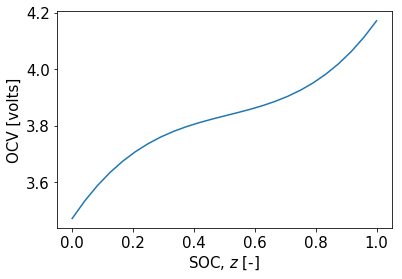
\includegraphics[width=20em]{"imgs/[1] HW1"/7a.png}
    \caption{SOC vs. OCV}
    \label{fig:7a}
\end{figure}


\item Compared to the starter code I flipped the order of equations in the matrix stacking so I had to edit the given parts somewhat to match. 

\begin{figure}
    \centering
    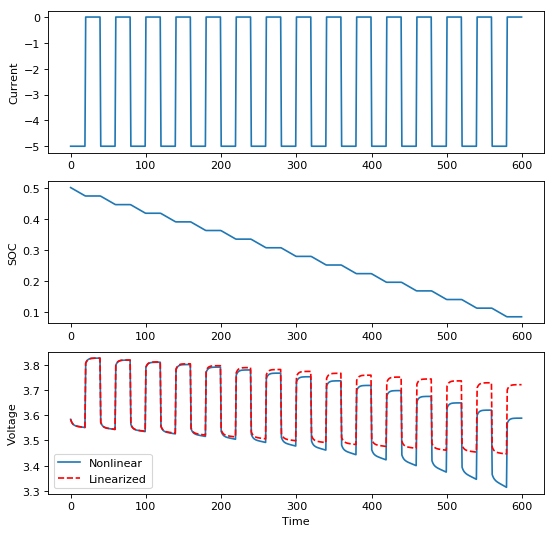
\includegraphics[width=20em]{"imgs/[1] HW1"/7b.png}
    \caption{Current, SOC, and voltage over time}
    \label{fig:7a}
\end{figure}

\item Below 0.25 SOC, the negative relationship between SOC and OCV accelerates away from a linear-like trend downward to a somewhat quadratic curve, dropping the true voltage more aggressively than the linear model can capture. This makes clear the limitations of a linear model to capture trends that deviate strongly from any sort of straight line, and optimization or control done on these linear models run the risk of not operating correctly on the true system, as may be evidenced by this battery voltage example.

\end{enumerate}

\end{Problem}

\end{document}
